\documentclass{article}
\usepackage{graphicx}
\usepackage[margin = 1.2in]{geometry}
\usepackage{amsmath}
\usepackage{epstopdf}

\begin{document}

For the following system of ODE's,

\begin{equation}
  \label{eq:sys}
  \begin{array}{l c l}
    c' &=& -\frac{\mu}{y} \frac{cx}{k_1 +c} - \frac{\eta}{y} \frac{cax}{k_2 +c} + q(c_0 - c) \\
    a' &=& -\frac{\eta}{z} \frac{cax}{k_2+c} + q (a_0 -a)\\
    x' &=& \mu \frac{cx}{k_1+c} - \eta \frac{cax}{k_2+c} - qx\\
    p' &=& \mu \frac{cx}{k_1 +c} + \eta \frac{cax}{k_2+c},
  \end{array}
\end{equation}


using the following parameter values,

\begin{center}
  \begin{tabular}{c|c}
    Parameter & Value \\
    \hline
    $\mu$ & 2 \\
    $y$ & 1\\
    $k_1$ & 1.5\\
    $k_2$ & 1.5\\
    $\eta$ & 20 \\
    $q$ & 0.3 \\
    $c_0$ & 1\\
    $a_0$ & 1\\
    $z$ & 1,
  \end{tabular}
\end{center}

I graphed out how the system behaves when the antibiotics, $a$, are introduced. To simulate this effect, the equation for $a'$ was changed to

\begin{equation}
  \begin{array}{llcl}
    &\alpha' &=& -\frac{\eta}{z} \frac{cax}{k_2+c} + q (-a + a_0 [h(t_{start},t) - h(t_{end},t)]), \\
    \text{where }& h(x,y) &=& \frac{x^n}{y^n + x^n}, \\
    &t_{start} &=& 4, \\
    &t_{end} &=& 8,\\
    \text{and }&n &=& 150. 
  \end{array}
\end{equation}

With this change we have that $\alpha'(x) = a'(x), \forall x, 4 \le x \le 8$. The graphs can be seen in Figure \ref{eqsVsTime} and in Figure \ref{phase:xc}.


\begin{figure}
  \centering
  \begin{tabular}{cc}
    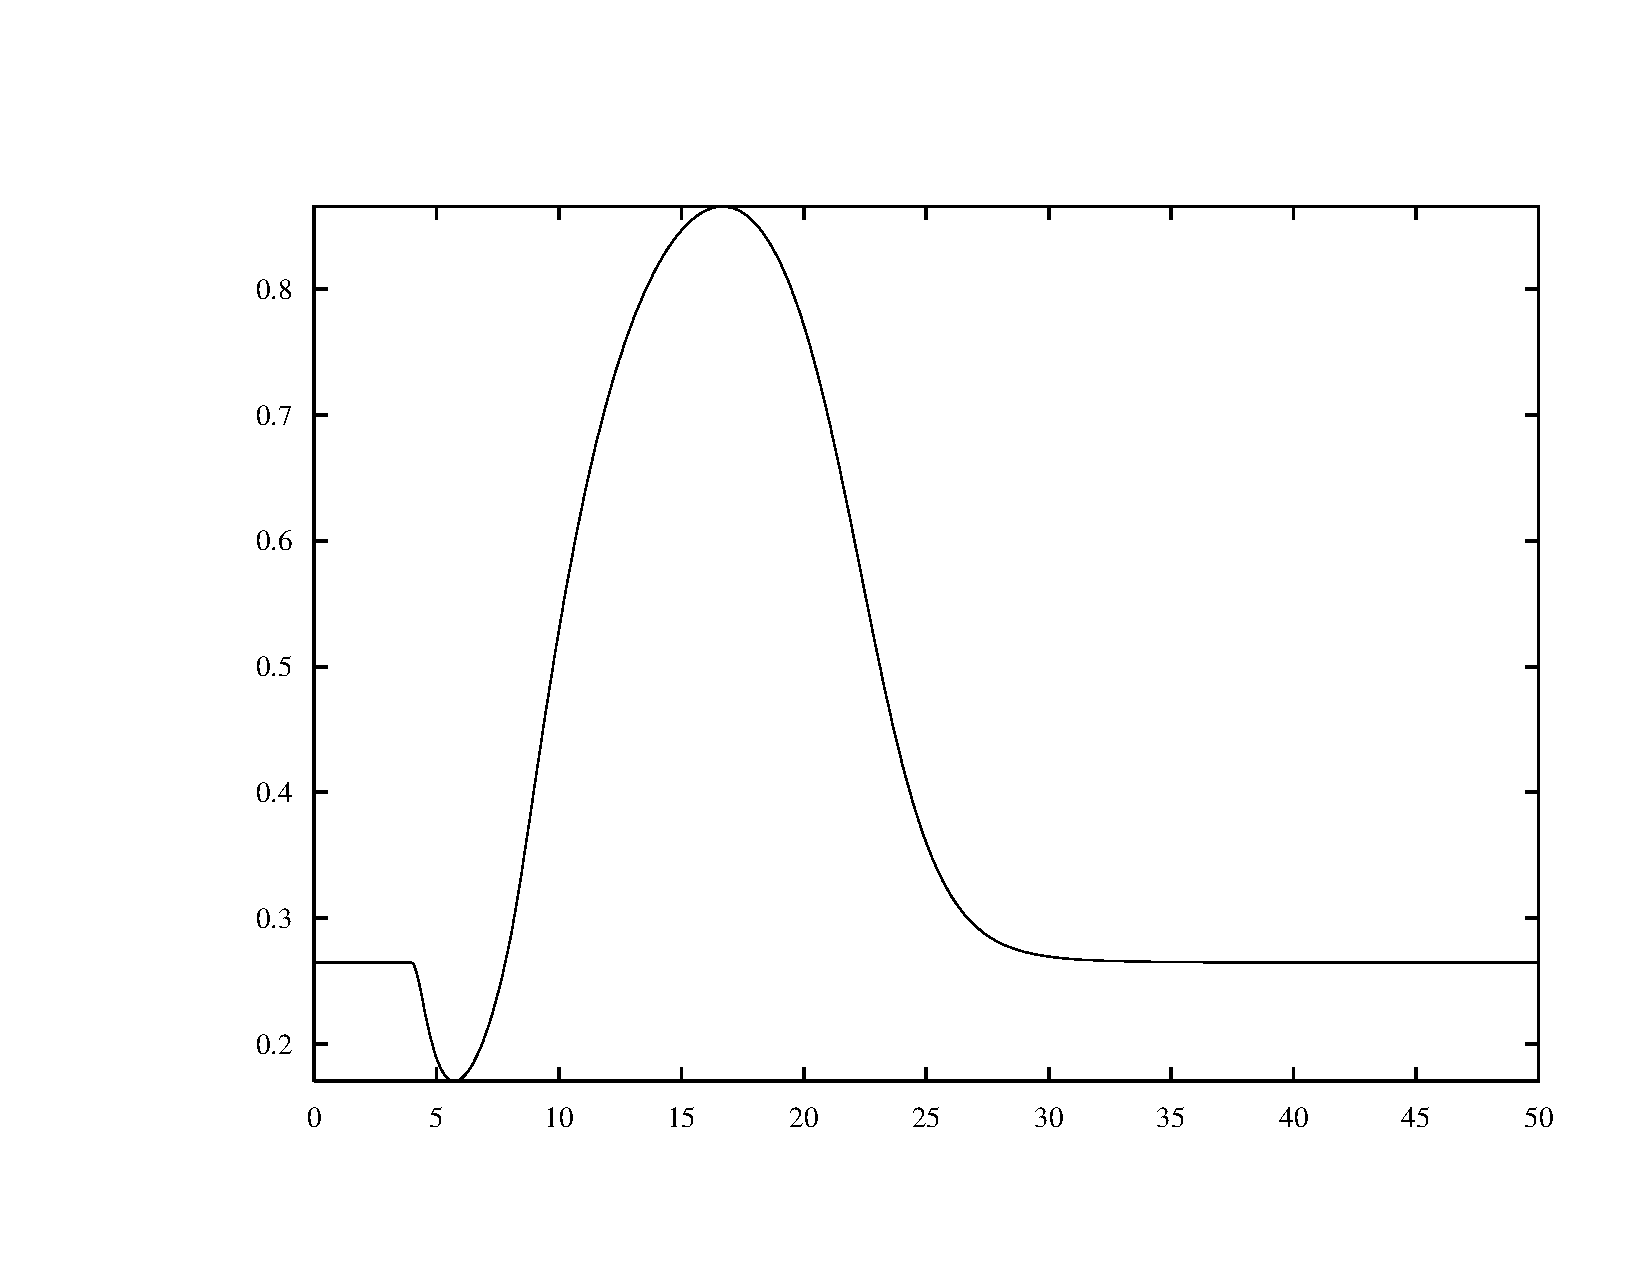
\includegraphics[scale = 0.23, angle = 0]{carbonTime.pdf} &
    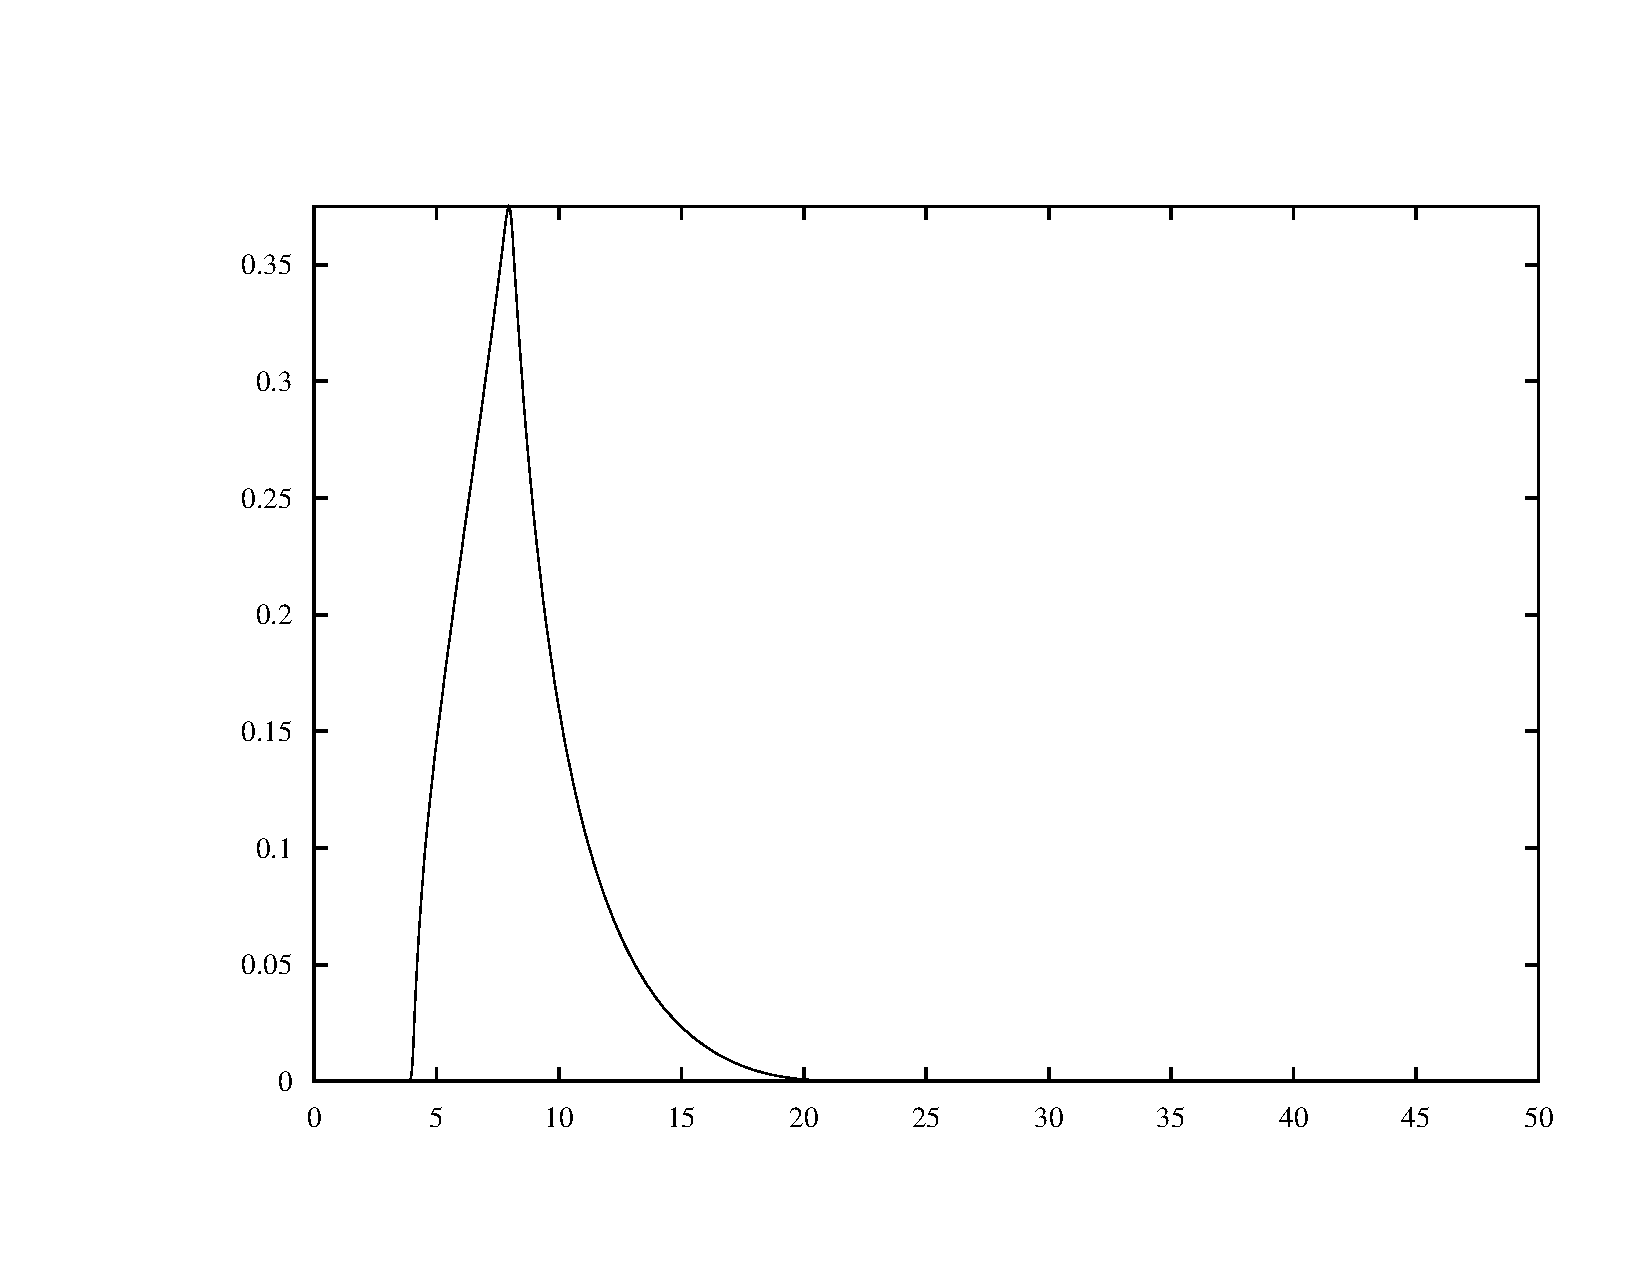
\includegraphics[scale = 0.23, angle = 0]{antiTime.pdf}  \\
    (a) & (b) \\
    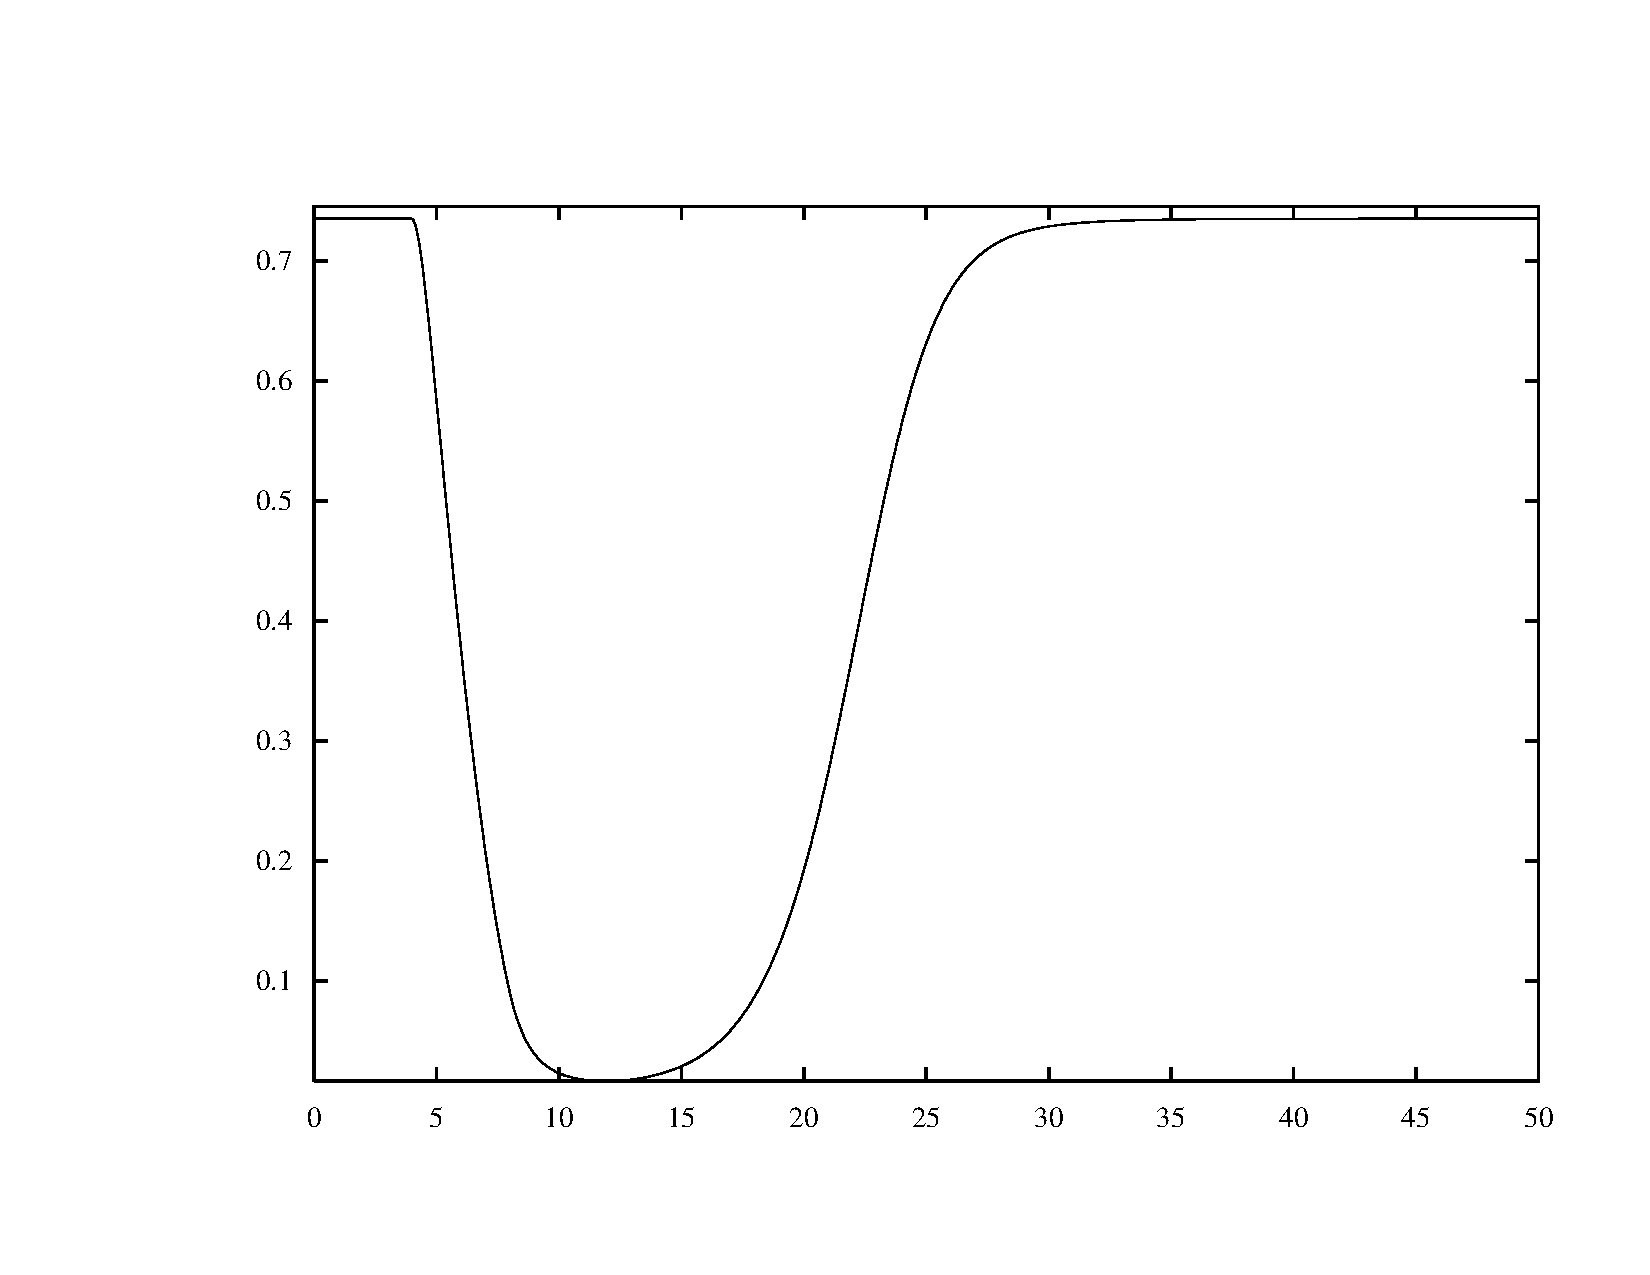
\includegraphics[scale = 0.23, angle = 0]{bactTime.pdf} &
    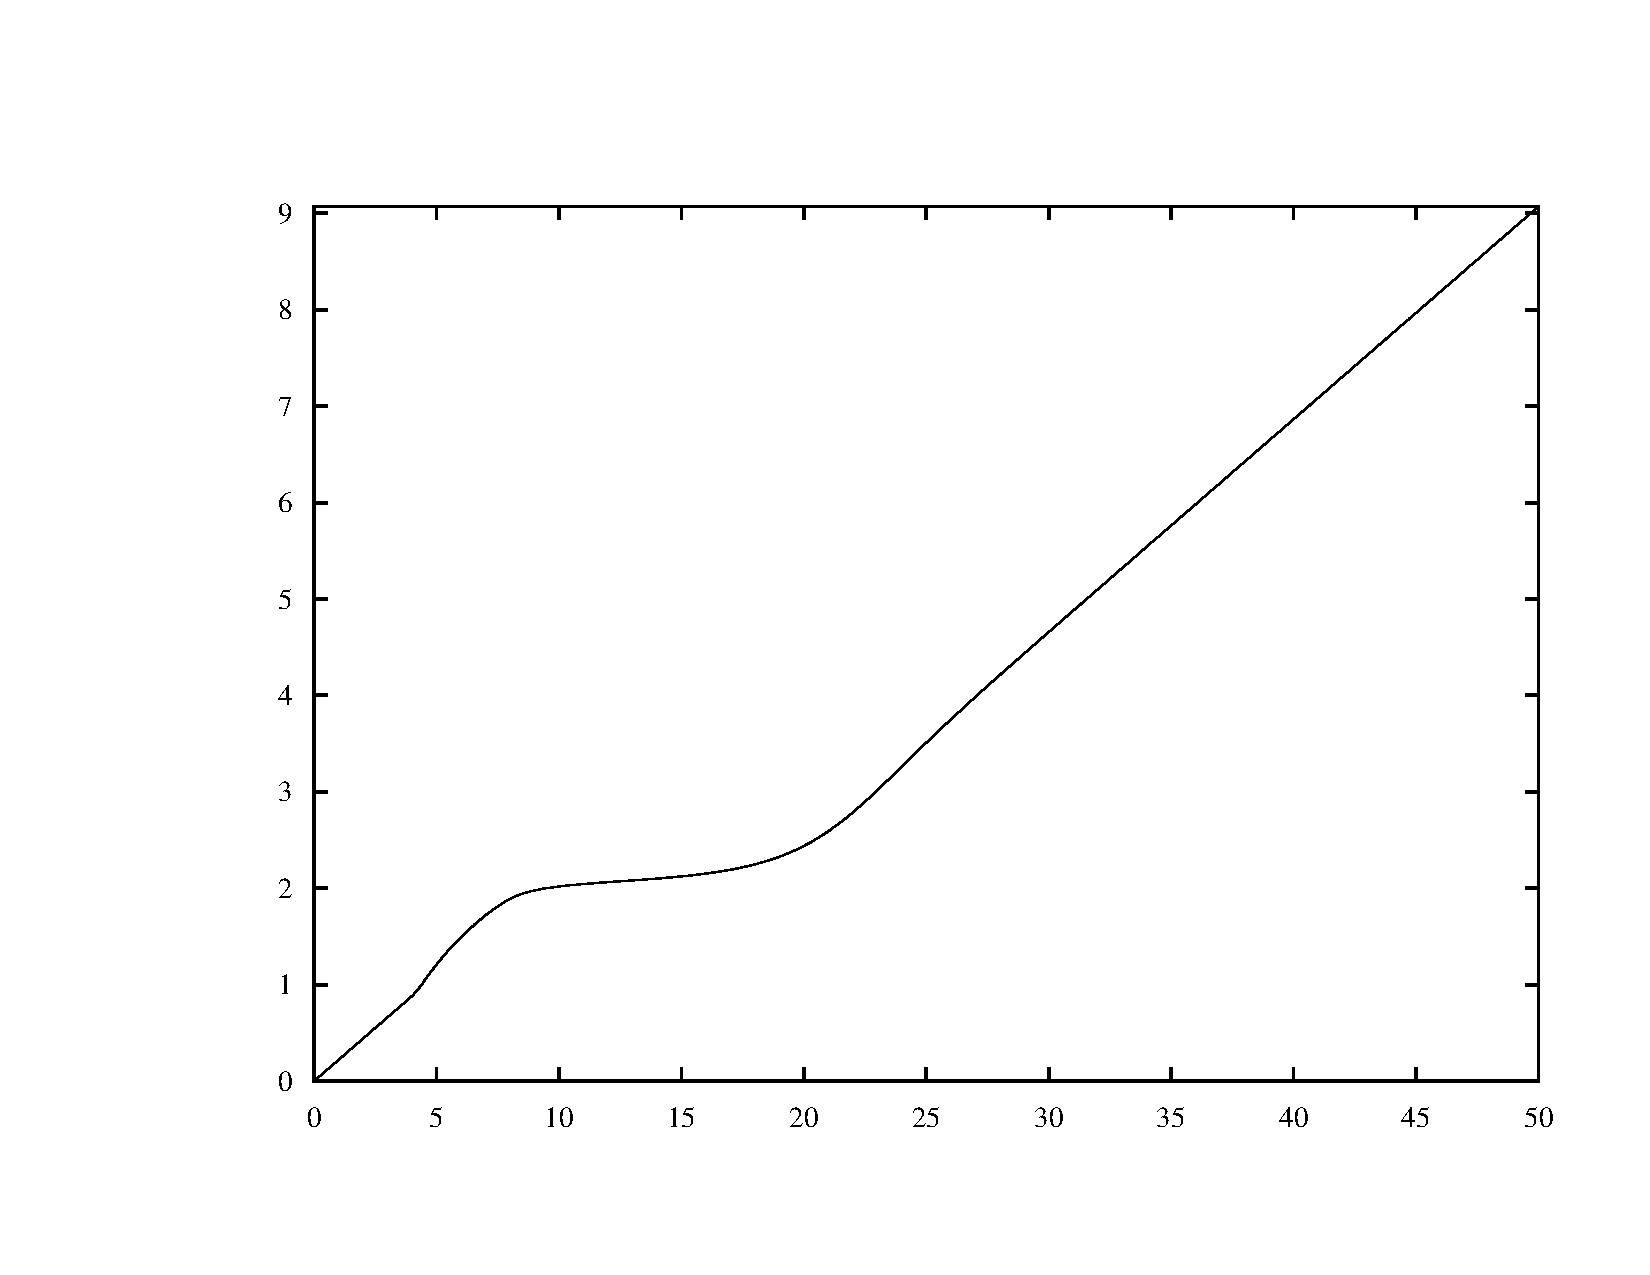
\includegraphics[scale = 0.23, angle = 0]{biprodTime.pdf}\\
    (c) & (d)
  \end{tabular}
  \caption{(a) $c$ vs. time, (b) $a$ vs. time, (c) $x$ vs. time, and (d) $p$ vs. time}
  \label{eqsVsTime}
\end{figure}



\begin{figure}
  \centering
  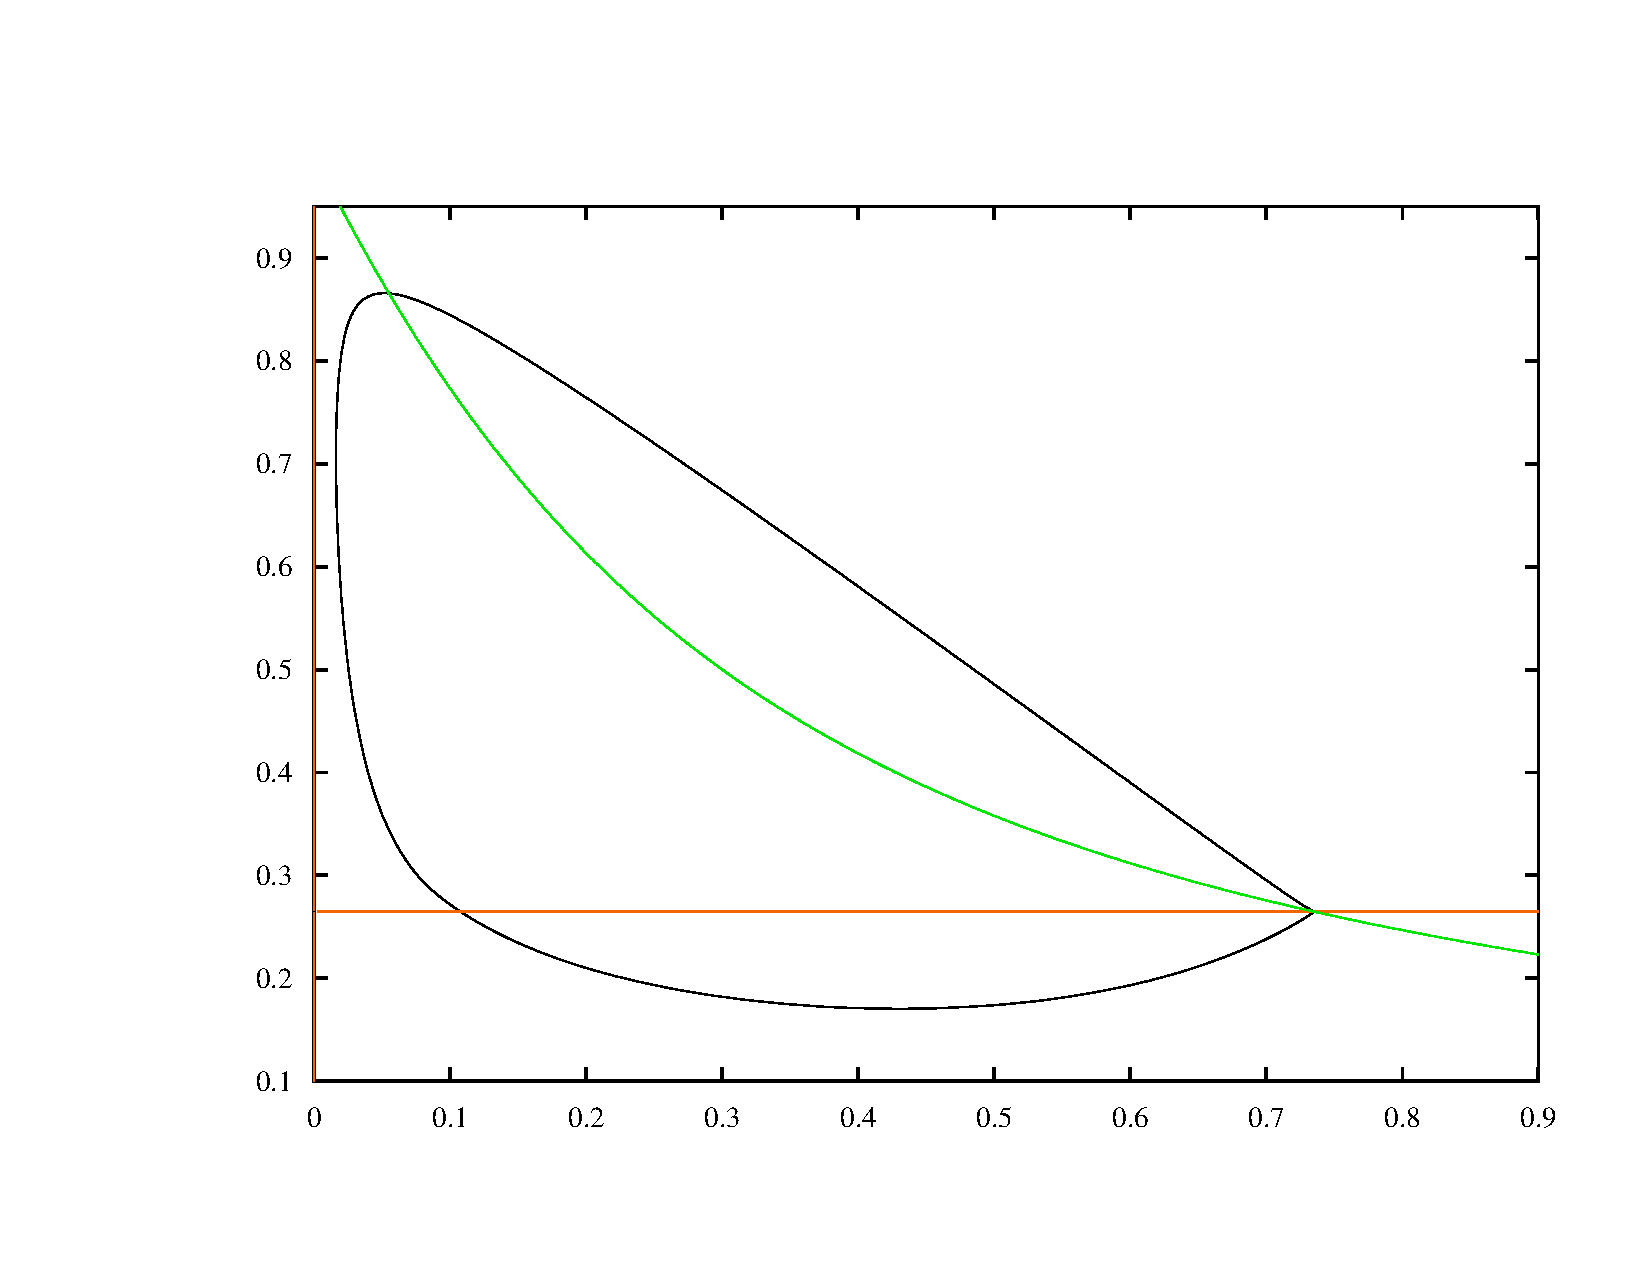
\includegraphics[scale = 0.35]{carbonBact.pdf}
  \caption{Phase portrait of $x$ and $c$}
  \label{phase:xc}
\end{figure}


The effect of replacing $\frac{cax}{k_2 +c}$ with $\frac{k_2 cax}{(k_1+c)(k_2+c)}$ in (\ref{eq:sys}) was again examined. As before, it was determined that there is no noticable effect from this change.

A plot of how $p'$ changed with time can be seen in Figure \ref{plot:tp'}.

\begin{figure}
  \centering
  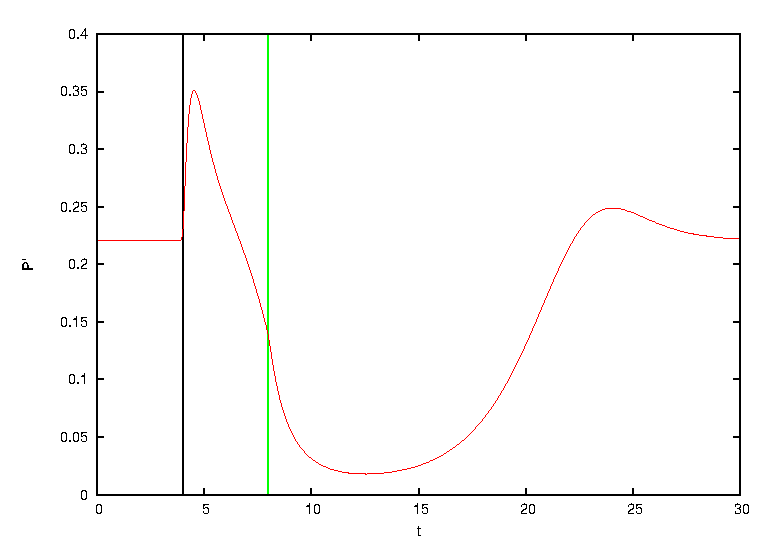
\includegraphics[scale = 1]{timePprime.eps}
  \caption{Plot of $p'$ vs. time. The black line indicated when the antibiotics are introduced into the system, the green line shows the time they stopped.}
  \label{plot:tp'}
\end{figure}



\end{document}




